\chapter{Image guided radiation therapy and computed tomography}\label{ch:soa}

This chapter explores the relevant state of the art for the work in this thesis. First, a short introduction of the technique used in IGRT, specially in lung IGRT is presented, with focus in the lung imaging. This shows how CBCT is a widely used technique in IGRT and how dealing with motion is key in IGRT. Then a small introduction of other uses of CBCT is presented. Later, CERN's phase space tomography, and its motion compensation method is described. The techniques used for removing motion in CERN's proton synchrotron is the base for the methods presented in chapters 6 and 7. Finally, the relevant literature for dealing with motion in CBCT is presented.


\section{Image Guided Radiation Therapy}


Due to the lower doses used than in a conventional CT scan and to its slow data acquisition rate, a CBCT image is generally riddled with noise and motion artefacts. 
\section{CT imaging in other applications}

\section{Phase Space Tomography at the proton Synchrotron}

Motion in tomography is a problem not only in X-ray modalities. Phase space tomography is a hybrid algorithm that combines particle tracking in a computer model of a synchrotron with iterative algorithms to reconstruct an image of the population of a bunch of particles circulating in the accelerator. The particle motion involves non-linear rotation and is non-cyclic, but a 1D projection of the distribution can be completely acquired as a single snapshot on one turn of the machine. By tracking test particles to gain a knowledge of how the geometry of the 2D image plane (longitudinal phase space) deforms, the information in all the discrete time slices acquired over many turns can be translated back to the same instant and topographically combined in a single image. This is possible because the motion of this particles can be exactly known from understanding and measuring the physics involved int he particle acceleration process. To do so, each pixel in the reconstructed image is populated with a bunch (generally 16) phantom particles, and their movement is simulated. By knowing in which measurement bin each fraction of the pixels (each phantom particle) falls in each position in time, the tomographic reconstruction can be performed by assigning values to the locations of these particles in the desired time position. Figure \ref{fig:PST} shows the measured projections and reconstructed images using these technique. If the motion modelling were not included, the swirl pattern would not be visible.

\begin{figure}

\begin{center} 

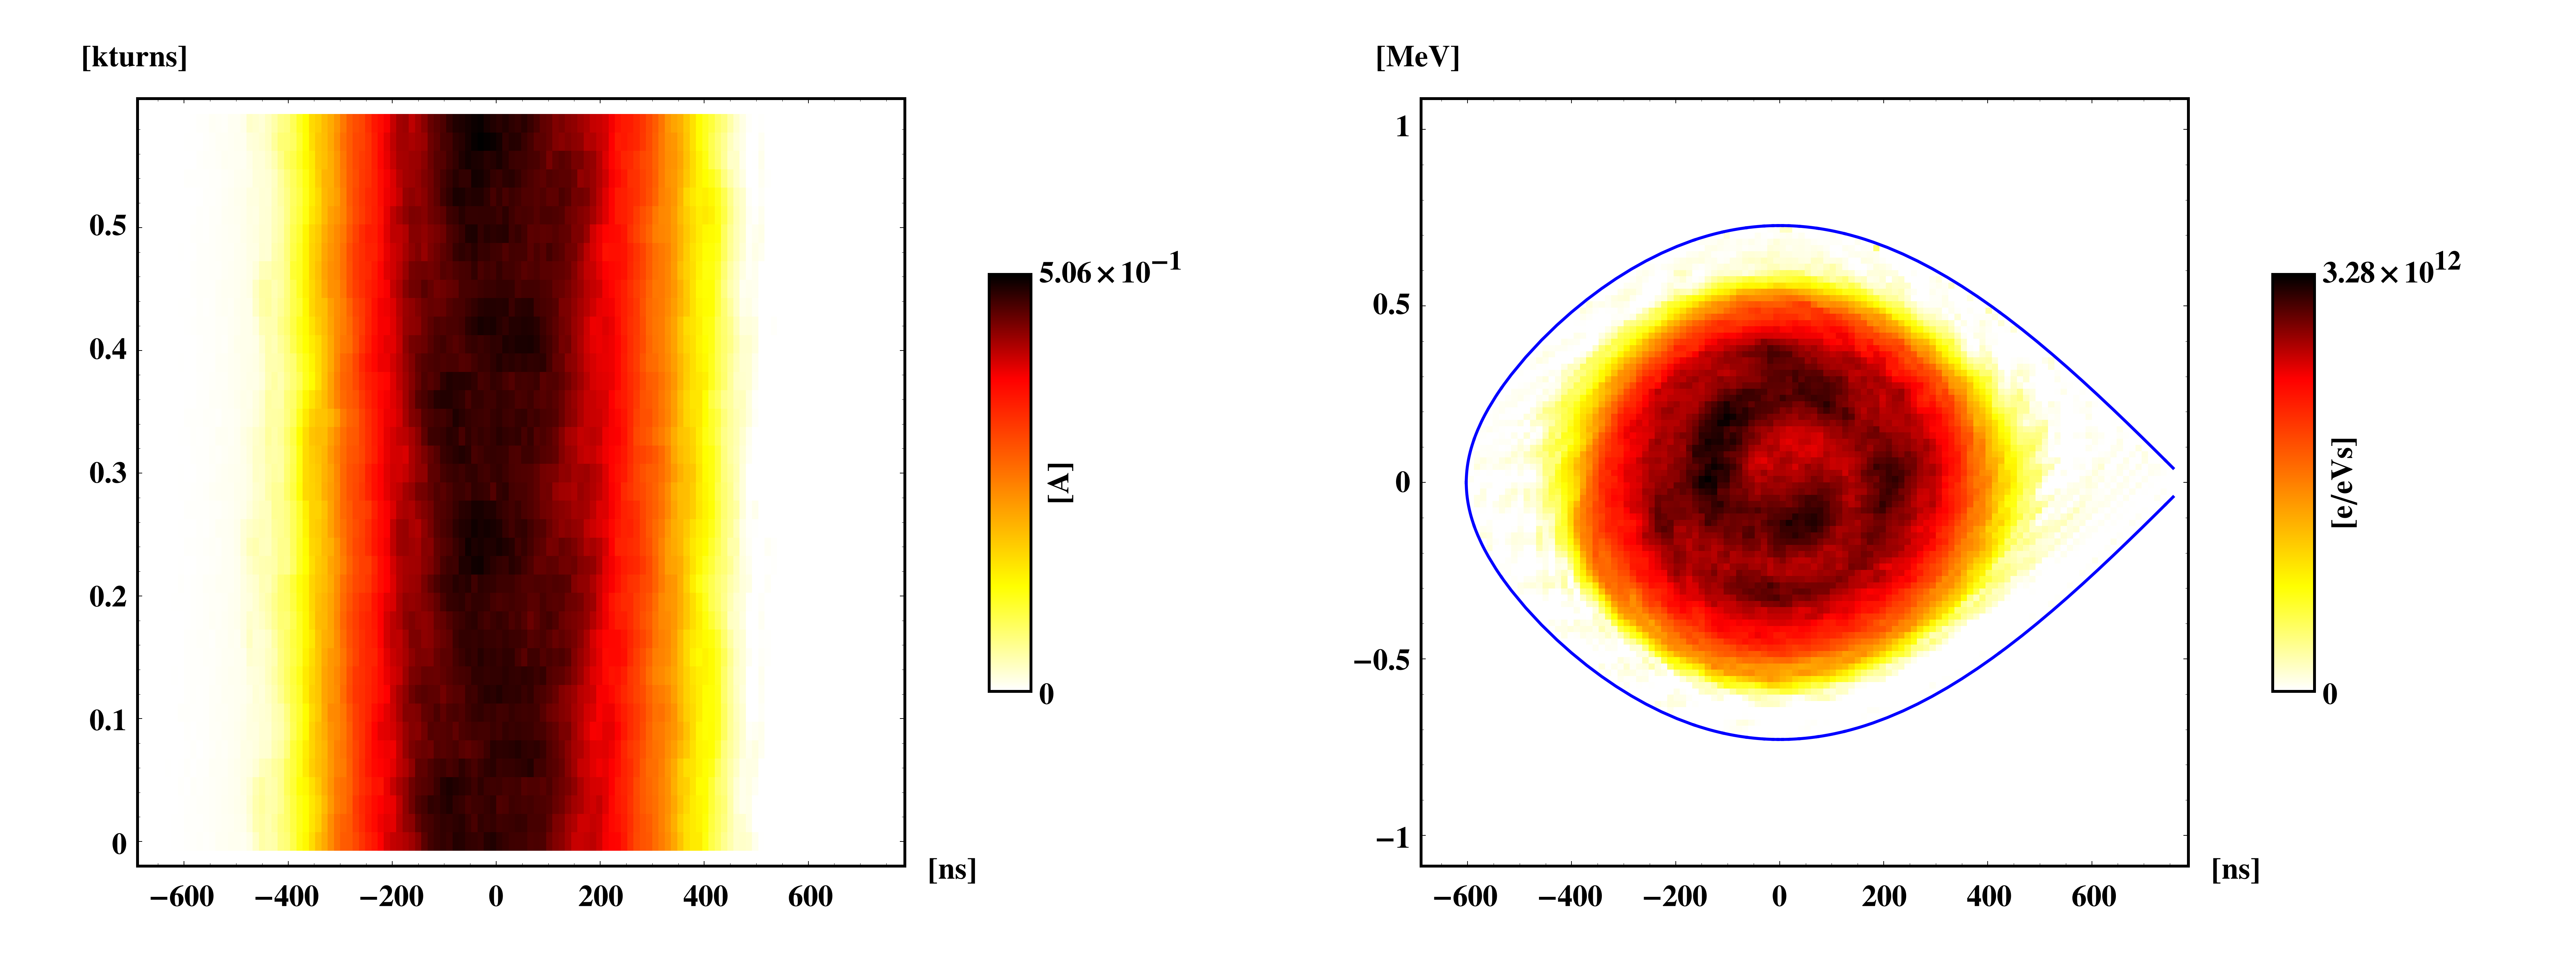
\includegraphics[width=\linewidth]{StateOfArt/Tosca2016fig.png} 

\caption[Phase space tomography]{\label{fig:PST} Early example (1999) of a set of 1D bunch profile data (left) processed into a 2D image of particle density in the longitudinal plane (right) using phase space tomography.  The resultant particle distribution is consistent with all the measured profiles and the physics of synchrotron motion.  The detailed internal bunch structure that is revealed is a consequence of the non-linearity of the motion.  The measurement was made at the CERN Proton Synchrotron Booster.\cite{pstweb}.} 
\end{center} 
\end{figure}


 Conceptually the method means adding the motion information to the geometry of the model with which the problem is posed rather than inserting it somehow into the mathematics of the tomography by which a solution is found. However, the specific technique used in phase space tomography is not viable in medical imaging, as the images are already very big in pixels, increasing the size e.g. 16 times would be computationally infeasible. Thus, the concept of phase space tomography must be implemented using a different method in CBCT.

\section{Motion in CBCT}
 Research into the removal of motion artefacts in CBCT is widespread and numerous articles have been published on the subject.  The most studied method to deal with motion is phase-correlated CBCT, also called 4D-CBCT\cite{sonke2005respiratory}\cite{thomas2006}\cite{li2006four}\cite{Pengpan2012246}\cite{t2016first}.  In 4D-CBCT, projection data are binned according to respiratory phase and then the data from each bin are reconstructed separately to produce a series of images.  This approach has several drawbacks.  Even though the amount of data per reconstructed image is smaller than usual, the total number of projections increases which means a longer irradiation time and a higher dose for the patient, limiting its clinical use.  In addition, the image quality of each 4D-CBCT reconstruction is inferior to a 3D-CBCT one due to its reduced angular sampling and to small inconsistencies resulting from binning inaccuracies. 

Due to the limitations of standard 4D-CBCT imaging, extensive research has been conducted to improve the quality of the images.  This work can be divided into two main groups: algorithmic approaches and deformation vector field (DVF) optimization methods.  Methods in the first group rely on regularization and other similar approaches.  An example is the work by Jia \textit{et al.}\cite{jia2012}, who implemented a non-local means of reconstruction to improve the temporal similarity between images.  Total variation methods (TV)\cite{ASD_POCS}, which minimize gradients within an image, have been also proposed with a temporal dimension included in the gradient\cite{0031-9155-57-6-1517}.  Another method based on TV minimization is the so-called PICCS algorithm\cite{chen2008prior}\cite{0031-9155-53-20-006}\cite{chen2012time} (it is actually a regularizer), which minimizes the TV and the difference between the reconstructed image and a prior image.  This prior image is generally a CBCT reconstructed with motion artefacts.  PICCS can reconstruct 4D-CBCT images from highly undersampled datasets.  More complex algorithms have also been proposed, such as ROOSTER\cite{:/content/aapm/journal/medphys/41/2/10.1118/1.4860215}, where a series of regularizations and minimizations are performed inside a region of interest to create clear 4D images in that area.

The methods of the second group generally (but not always) rely on a previous high-quality 4D-CT treatment planning scan as the basis from which to compute the DVFs.  As breathing motion is neither truly periodic nor reproducible in a given patient over time, the DVFs are corrected by matching real projections with simulated ones.  Finally, when the best DVF is computed, a synthetic image is generated by deforming the prior high-quality CT scan.  Examples include the work of Brock \textit{et al.}\cite{brock2010} and Ren \textit{et al.}\cite{Ren20121584}, who managed to reduce the number of projections required to about 60 using non-linear conjugate-gradient methods.  In order to improve robustness and reduce the dimensionality of the problem, DVF principal component analysis methods have also been proposed\cite{zhang2010correction}.  Li \textit{et al.}\cite{:/content/aapm/journal/medphys/37/6/10.1118/1.3426002}\cite{:/content/aapm/journal/medphys/38/5/10.1118/1.3582693} demonstrated that good accuracy can be achieved using only a single projection for the DVF optimization.

Hybrids between DVF-based and algorithmic approaches also exist, such as using TV regularization methods to improve convergence by initializing the DVFs\cite{wang2012high} or using temporal regularization with DVFs to improve the ROOSTER algorithm\cite{mory2016motion}.  Hybrid methods can lead to highly complex optimization strategies.  Examples include segmented mesh-based 4D-CBCT\cite{0031-9155-61-3-996} and the separation of static and moving images using TV, tight frame regularization and DVF optimization\cite{0031-9155-56-11-002}.  In addition, Christoffersen \textit{et al.}\cite{christoffersen2013registration} have proposed a multi-step algorithm using TV and optical flow for motion estimation.

Finally, some special mathematical algorithms have also been suggested that are unique in their approach.  These include the cine-CBCT algorithm\cite{6803058} and the 5D motion modelling approach\cite{0266-5611-31-11-115007}, which does not use phase-correlated binning.

The literature is full of these and many other approaches, ranging from the computationally and mathematically complex to those that sacrifice accuracy for simplicity and speed.  Most have been shown to yield good 4D-CBCT reconstructions, some in clinical scenarios.  But they all have drawbacks.  CBCT is a severely ill-posed problem where the amount of data is key for a good reconstruction.  The simplest methods that rely on binning will always suffer to some extent from a lack of data, even if temporal coherence is enforced with mathematical norms.  Additionally, they involve the reconstruction of several images, which is very expensive both computationally and in terms of memory.

Most DVF-based approaches ultimately use the DVFs to deform a prior image rather than using the acquired data directly to produce a reconstruction.  Further, they assume that a DVF can describe every possible anatomical change with respect to that prior image and this does not necessarily hold.

%{red}{\sout{Here, we propose a completely different approach to motion compensation in 4D-CT imaging.}}
In this work, a modelling method for motion compensation is presented, as first proposed by Hancock \textit{et al.}\cite{pst1} outside the medical domain and later independently proposed by Rit \textit{et al.}\cite{Rit1}\cite{Rit2} for CBCT. Since the publication of their work, computing on graphical processing units (GPUs) has taken a significant leap forward affording more modern techniques that can be used to reconstruct with greater accuracy and computational efficiency. With the use of GPUs even generic motion compensation is possible, without any numerical approximation of the weights in the projection and back projection and using better forward modelling\cite{fwdproj}. Such an approach is presented in this work.

This thesis focuses on thorax CBCT, but the method is generalizable to any X-ray absorption CT modality and to arbitrary motion.  The method requires no binning, but instead uses all projections to reconstruct an image at any respiratory phase.  It does require a sufficiently accurate description of the motion in terms of DVFs, but the approach is a modelling one so it can be used to introduce motion compensation into any iterative reconstruction algorithm. 

\section{Discussion}

Hopefully the topics presented in this chapter clarify why motion is a key problem to solve in IGRT and hadron therapy, and the solution should start by being able to image in 4D. The concepts in phase space tomography not only can potentially solve the problem, but can do so by reducing the amount of data acquired significantly. This concept has been barely explored in the literature. Additionally, any general improvement on image quality in CBCT would not only benefit medical applications, but a entire set of different uses of the imaging technology.